\documentclass{standalone}
\usepackage{tikz} % Import the tikz package
\usetikzlibrary{automata} % Import library for drawing automata
\usetikzlibrary{positioning} % ...positioning nodes
\usetikzlibrary{arrows} % ...customizing arrows
\tikzset{node distance=2.5cm,
    every state/.style={
        semithick,
        fill=gray!10},
    initial text={},
    double distance=2pt,
    every edge/.style={
        draw,
        ->,>=stealth',
        auto,
        semithick}}
\let\epsilon\varepsilon
\begin{document}
    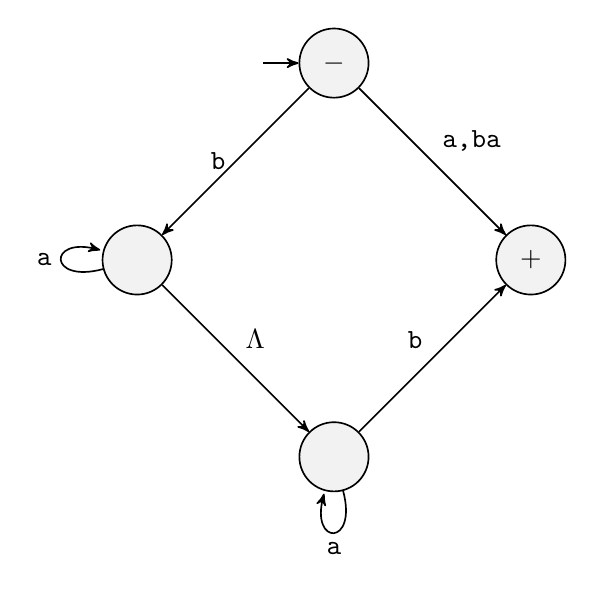
\begin{tikzpicture}
        \node (mid) {};
        \node[state,initial,above of=mid] (q1) {$-$};
        \node[state, left of=mid] (q2) {};
        \node[state, below of =mid] (q3) {};
        \node[state, right of=mid] (q4) {$+$};
        \draw (q1) edge[left] node {\tt b} (q2);
        \draw (q1) edge node {\tt a,ba} (q4);
        \draw (q2) edge[loop left] node {\tt a} (q2);
        \draw (q2) edge node {\tt $\Lambda$} (q3);
        \draw (q3) edge[loop below] node {\tt a} (q3);
        \draw (q3) edge node {\tt b} (q4);
    \end{tikzpicture}
\end{document}